\subsection{DEM - Distinct-Element-Method}
\index{DEM Distinct Element Method}

The distinct element method (DEM) extends the capabilities of continuum-mechanical approaches by introducing 
a new level of discretization, which allows it to describe independent deformable bodies that can interact 
via their contact points and surfaces, see Fig. \ref{fig:demskizze}. The behaviour of these contacts can be modelled using joint constitutive models, which are typically formulated in terms increments. This approach is especially suitable for materials with a pronounced grain structure, such as salt rocks. 

\begin{figure}[!ht]
\centering
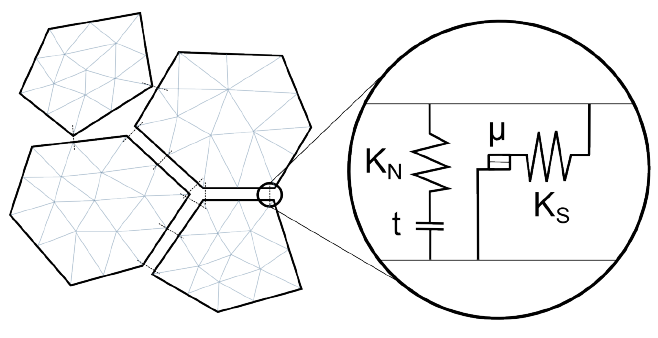
\includegraphics[width=0.6\textwidth]{figures/skizze.png}
\caption{Interaction between blocks and contacts in the DEM}
\label{fig:demskizze}
\end{figure}

The models of rock salt, from laboratory scale samples to entire potash mines, therefore need to be built from 
randomised assemblies of polyhedral grains, in order to simulate the discontinuous and granular nature. The generation of the randomised structures is based on Voronoi-discretization, which allows to divide arbitrary volumes (areas) into polyhedral parts. The program generates pseudo-random point clouds using a Monte-Carlo-method, which can then be refined to avoid clustering. It is also possible to introduce a local variation of the grains size this way. 
The thermo-hydro-mechanical behaviour of a model set up in this way is then a combination of the behaviour of the 
bulk of the grains, and of the contact properties. For both, constitutive laws were derived at IfG. 
\index{Voronoi tessellation}

Since it would be computationally unfeasible to represent a large geological structure with realistic grain sizes 
of millimeters or centimeters, a coarse-grained approach is taken. This approach was validated by carrying out 
discretization studies with a variation of Voronoi sizes. The blocks/grains dominate the hardening and the creep 
behaviour, while the softening occurs predominantly by shear and tensile failure on grain boundaries. 

Another advantage of the discontinuum mechanical approach lies in its capabilities to model the pressure driven 
percolation of gases and fluids on discrete flow paths on opened grain boundaries. The undamaged grain boundaries 
start out as impermeable but can be opened due to plastic failure. 

The constitutive laws for both bulk and contacts were implemented as DLLs for the programs UDEC and 3DEC of Itasca CG, Inc.
